\section{Expériences avec \beagle}
\subsection{Software, hardware et tests}
\beagle est en cours de dévellopement et nos tests ont utilisés la version 0.7 de \beagle.
 Ces expériences ont été menés sur un processeur deux coeurs cadencées à 2.1Ghz avec 3,7 GB de mémoire vive. Les problèmes testés sont les 271 premiers problèmes que \metis résout lors de la construction de \holfour.

\subsection{Présentation de \beagle}
\beagle est prouveur automatique supportant le premier ordre, les types monomorphes et l'arithmétique. sur les problèmes arithmétiques. Il accepte en entrée des problèmes au format \tff. Des résultats expérimentaux(sur une version obsolète) ainsi que la théorie détaillée de \beagle peuvent être trouvés dans ~\cite{Waldmann13}.


\subsection{Impact de la monomorphisation}

\noindent \begin{tabularx}{\textwidth}{|X|X|}
\hline
Avant monomorphisation & Après monomorphisation \\
\hline
\begin{tikzpicture}[scale=1.5]
    \slice{0/100*360}
          {70/100*360}
          {70\%}{insatisfaisable}{green}
    \slice{70/100*360}
          {84/100*360}
          {14\%}{satisfaisable}{red}      
    \slice{84/100*360}
          {91/100*360}
          {7\%}{inconnu}{red}
    \slice{91/100*360}
          {99/100*360}
          {8\%}{time out}{red}
    \slice{99/100*360}
          {100/100*360}
          {1\%}{parsing error}{red}                            
\end{tikzpicture}
&
\begin{tikzpicture}[scale=1.5]
    \slice{0/100*360}
          {80/100*360}
          {80\%}{insatisfaisable}{green}
    \slice{80/100*360}
          {81/100*360}
          {1\%}{satisfaisable}{red}  
    \slice{81/100*360}
          {86/100*360}
          {5\%}{inconnu, yshift=6}{red}   
     \slice{86/100*360}
           {98/100*360}
           {12\%}{time out}{red}     
     \slice{98/100*360}
           {100/100*360}
           {2\%}{parsing error}{red}               
\end{tikzpicture}
\\
\hline
\end{tabularx}
Commentaires des erreurs.

\subsection{Utilisation des différentes étapes de la traduction}

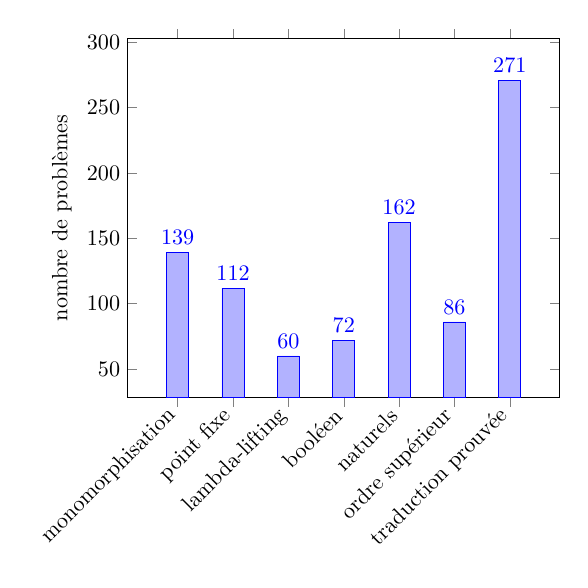
\begin{tikzpicture}[scale=0.8]
\begin{axis}[ybar,enlargelimits=0.15,legend style={at={(2,2)},anchor=north,legend columns=0},ylabel={nombre de problèmes},symbolic x coords={monomorphisation,point fixe,lambda-lifting,booléen,naturels,ordre supérieur,traduction prouvée},xtick=data,
nodes near coords,
nodes near coords align={vertical},
x tick label style={rotate=45,anchor=east},]
\addplot coordinates {(monomorphisation,139) (point fixe,112) (lambda-lifting,60) (booléen,72)(naturels,162)(ordre supérieur,86)(traduction prouvée,271)};
\end{axis}
\end{tikzpicture}


\subsection{Efficacité de \beagle}
A travers ses exemples, il est difficile de juger de la qualité de \beagle
face à \metis puisque \metis résout l'ensemble de ses buts rapidement.
Parmi les problèmes, nous avons retenu 69 problèmes contenant au moins un théorème donné par l'utilisateur contenant uniquement des constantes arithmétiques $+$,$-$,$\leq$,$<$,$\geq$,$>$ et nous avons supprimés 79 tels théorèmes. \metis n'est donc plus en mesure de résoudre l'un de ses problèmes modifiés. Cependant \beagletac y parvient:


\noindent \begin{tabularx}{\textwidth}{|X|X|}
\hline
Résultats & Utilisation du code \\
\hline
\begin{tikzpicture}[scale=1.5,baseline=(current bounding box.center)]
    \slice{0/100*360}
          {88/100*360}
          {88\%}{insatisfaisable}{green}
    \slice{88/100*360}
          {97/100*360}
          {9\%}{inconnu}{red}
    \slice{97/100*360}
          {100/100*360}
          {3\%}{time out}{red}
\end{tikzpicture}
&
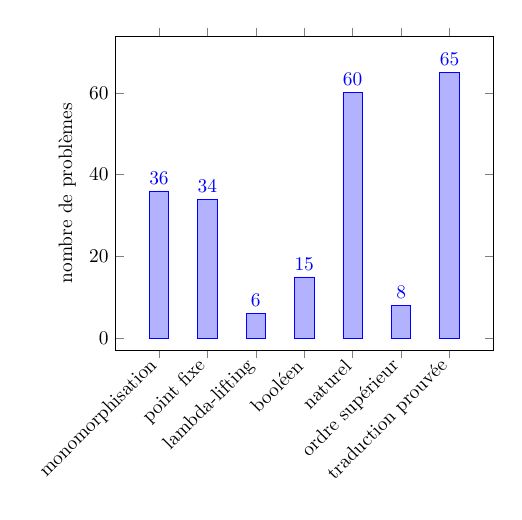
\begin{tikzpicture}[scale=0.7,baseline=(current bounding box.center)]
\begin{axis}[ybar,enlargelimits=0.15,legend style={at={(2,2)},anchor=north,legend columns=0},ylabel={nombre de problèmes},symbolic x coords={monomorphisation,
point fixe,lambda-lifting,booléen,naturel,ordre supérieur,traduction prouvée},xtick=data,
nodes near coords,
nodes near coords align={vertical},
x tick label style={rotate=45,anchor=east}]
\addplot coordinates {(monomorphisation,36) (point fixe,34) (lambda-lifting,6) (booléen,15)(naturel,60)(ordre supérieur,8)(traduction prouvée,65)};
\end{axis}
\end{tikzpicture}
\\
\hline
\end{tabularx}

De plus \beagle combine raisonnement du premier ordre et l'arithmétique, ce qui grâce à notre traduction permet à \beagletac de résoudre des problèmes combinant ordre supérieur et arithmétique.

